\documentclass[a4paper,12pt]{article} % тип документа

% Поля страниц
\usepackage[left=2.5cm,right=2.5cm,
    top=2cm,bottom=2cm,bindingoffset=0cm]{geometry}
    
%Пакет для таблиц   
\usepackage{multirow} 
    
%Отступ после заголовка    
\usepackage{indentfirst}

% Рисунки
\usepackage{floatrow,graphicx,calc}
\usepackage{wrapfig}

%%% Работа с картинками
\usepackage{graphicx}  % Для вставки рисунков
\graphicspath{{images/}}  % папки с картинками
\setlength\fboxsep{3pt} % Отступ рамки \fbox{} от рисунка
\setlength\fboxrule{1pt} % Толщина линий рамки \fbox{}
\usepackage{wrapfig} % Обтекание рисунков и таблиц текстом

% Создаём новый разделитель
\DeclareFloatSeparators{mysep}{\hspace{1cm}}

% Ссылки?
\usepackage{hyperref}
\usepackage[rgb]{xcolor}
\hypersetup{				% Гиперссылки
    colorlinks=true,       	% false: ссылки в рамках
	urlcolor=blue          % на URL
}


%  Русский язык
\usepackage[T2A]{fontenc}			% кодировка
\usepackage[utf8]{inputenc}			% кодировка исходного текста
\usepackage[english,russian]{babel}	% локализация и переносы

% Математика
\usepackage{amsmath,amsfonts,amssymb,amsthm,mathtools}

%%% Дополнительная работа с математикой
\usepackage{amsmath,amsfonts,amssymb,amsthm,mathtools} % AMS
\usepackage{icomma} % "Умная" запятая: $0,2$ --- число, $0, 2$ --- перечисление

% Что-то 
\usepackage{wasysym}


\begin{document}
\begin{center}
	\footnotesize{ФЕДЕРАЛЬНОЕ ГОСУДАРСТВЕННОЕ АВТОНОМНОЕ ОБРАЗОВАТЕЛЬНОЕ 			УЧРЕЖДЕНИЕ ВЫСШЕГО ОБРАЗОВАНИЯ}\\
	\footnotesize{МОСКОВСКИЙ ФИЗИКО-ТЕХНИЧЕСКИЙ ИНСТИТУТ\\(НАЦИОНАЛЬНЫЙ 			ИССЛЕДОВАТЕЛЬСКИЙ УНИВЕРСИТЕТ)}\\
	\footnotesize{ФИЗТЕХ-ШКОЛА ФИЗИКИ И ИССЛЕДОВАНИЙ им. ЛАНДАУ\\}
	\hfill \break
	\hfill \break
	\hfill \break
	\hfill \break
\end{center}

\begin{center}   
    \hfill \break
	\hfill \break
	\hfill \break
	\hfill \break    \hfill \break
	\hfill \break
	\hfill \break
	\hfill \break
    \hfill \break
    \hfill \break
	\hfill \break
	\large{Лабораторная работа № 2.2.1\\\textbf{Исследование взаимной диффузии газов}}\\
	\begin{flushright}
		Плотникова Анастасия Александровна\\
		Группа Б02-406
	\end{flushright}
	\hfill \break
	\hfill \break
	\hfill \break
\end{center}
\hfill \break
\hfill \break
\hfill \break
\hfill \break
\hfill \break
\hfill \break
\hfill \break
\hfill \break
\hfill \break
\hfill \break
\hfill \break
\hfill \break
\hfill \break
\begin{center}
	Долгопрудный, 2025 г.
\end{center}
\thispagestyle{empty}
\newpage
	\textbf{Цель работы:}\\ 
  1) регистрация зависимости концентрации гелия в воздухе от времени с помощью датчиков теплопроводности при разных начальных давлениях смеси газов;\\ 
  2) определение коэффициента диффузии по результатам измерений.
	\hfill \break
	
	\textbf{В работе используются:}\\ 
  измерительная установка;\\ 
  форвакуумный насос;\\ 
  баллон с газом (гелий);\\ 
  манометр;\\ 
  источник питания;\\ 
  магазин сопротивлений;\\ 
  гальванометр;\\ 
  секундомер.
	\hfill \break

\section*{Теоретическая справка}

\textit{Диффузией} называется самопроизвольное перемешивание молекул, происходящее вследствие их хаотичного теплового движения.

При перемешивании молекул разного сорта говорят о взаимной (или концентрационной) диффузии. 

Для наблюдения взаимной диффузии необходимо равенство давлений во всей системе (в противном случае возникнет гораздо более быстрое макроскопическое течение газа как сплошной среды).

\medskip

Пусть система состоит из двух компонетов a и b. 
Тогда плотность потока вещества любого компонента в результате взаимной диффузии определяется законом Фика. 

\begin{equation}
  j_a = - D_{ab} \frac{\delta n_a}{\delta x}, \quad j_b = - D_{ba} \frac{\delta n_b}{\delta x}
\end{equation}
где $D_{ab} = D_{ba} = D$ — коэффициент взаимной диффузии компонентов,\\ а $j_{a,b}$ — плотности потока частиц соответствующего сорта.

Исследуется диффузия примеси гелия на фоне воздуха. В условиях опыта $n_{\text{возд}} \gg n_{He}$, относительное изменение концентрации воздуха в результате взаимной диффузии мало. С достаточной точностью будем описывать только диффузию гелия на фоне воздуха. Далее $n = n_{He}$.

\section*{Экспериментальная установка}

Схема установки изображена на рисунке (\ref{fig:dr1}). 

\begin{figure}[h]
  \centering
  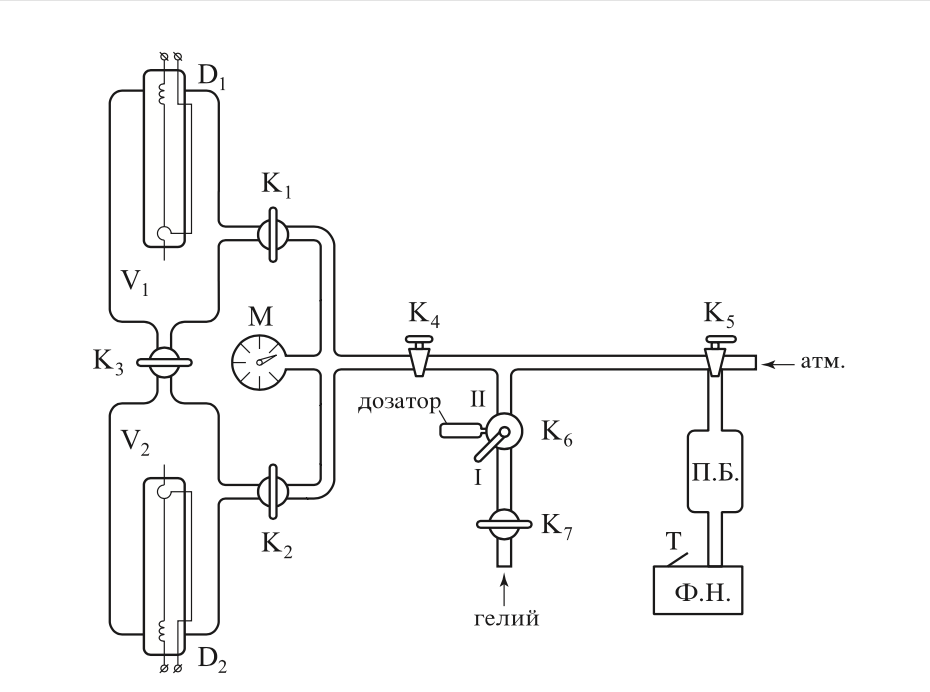
\includegraphics[scale = 0.75]{drawing1.png}
  \label{fig:dr1}
  \caption{Установка для исследования взаимной диффузии газов}
\end{figure}

Два сосуда с объёмами $V_1$ и $V_2$ соединены трубкой длины $l$ и сечения $S$. Сосуды заполнены смесью двух газов при одинаковом давлении, но с различной концентрацией компонентов. Вследствие взаимной диффузии концентрации каждого из компонентов в обоих сосудах с течением времени выравниваются.

Если бы концентрации в сосудах V1 и V2 поддерживались постоянными и равными n1 и n2, то в трубке установился бы стационарный поток частиц $J = - DS \frac{\delta n}{\delta x}$, одинаковый в каждом сечении трубки. Следовательно, $n(x)$ была бы линейной функцией координаты и $\frac{dn}{dx} = \frac{\Delta n}{l}$, где $l$ — длина трубки, откуда получаем

\begin{equation}
  J = - DS \frac{n_1 - n_2}{l} 
\end{equation}
\begin{equation}
  V_1 \Delta n_1 = - V_2 \Delta n_2 = J \Delta t = - DS \frac{n_1 - n_2}{l} \Delta t
\end{equation}
\begin{equation}
  V_1 \frac{dn_1}{dt} = - DS \frac{n_1 - n_2}{l}, \quad V_2 \frac{dn_2}{dt} = DS \frac{n_1 - n_2}{l}
\end{equation}
\begin{equation}
  \frac{dn_1}{dt} - \frac{dn_2}{dt} = - \frac{n_1 - n_2}l DS (\frac1{V_1} + \frac1{V_2})
\end{equation}

Введем новую переменную $\Delta n = n_1 - n_2$:
\begin{equation}
  \Delta n = \Delta n_0 e^{-t/\tau}
\end{equation}



\section*{Ход эксперимента}

\begin{enumerate}
  \item
\end{enumerate}

\section*{Обработка результатов измерений}

\begin{table}[h]
  \caption{}
  \begin{tabular}{|c|c|c|}
      \hline $T$, $^\circ C$  &  $\Delta h$, мм & $P$, Па \\
      \hline  &  &  \\
      \hline  &  &  \\
      \hline  &  &  \\
      \hline  &  &  \\
      \hline  &  &  \\
      \hline  &  &  \\
      \hline  &  &  \\
      \hline  &  &  \\
      \hline  &  &  \\
      \hline  &  &  \\
      \hline 
  \end{tabular}
  \label{tab:}
\end{table}

\section*{Вывод}
\end{document}
